%% ================================================================================
\chapter{Theory}
\label{ch:theory}
%% ================================================================================
The theory chapter. These are references \cite{aPaper}, \cite{aThesis}, \cite{aWiki}. Figure \ref{fig:dummy} shows a placeholder. 

\begin{figure}
  \centering
  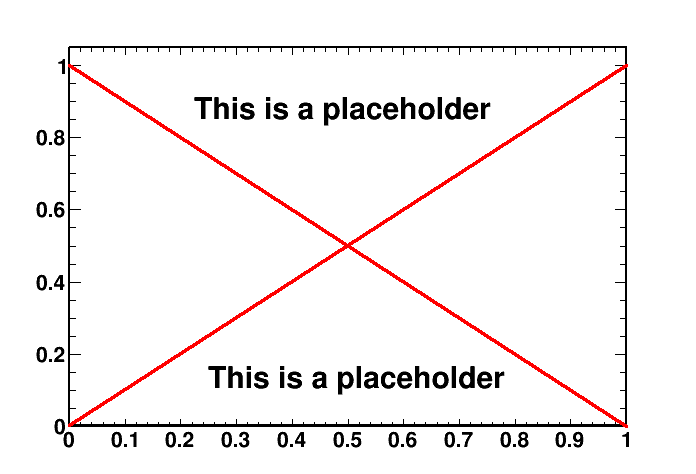
\includegraphics[width=.9\linewidth]{pic/dummy.png}
  \caption{This is a dummy plot.}
  \label{fig:dummy}
\end{figure}

\section{A section}
\label{sec:section}
Here we have Section \ref{sec:section}. \todo{This is a TODO marker} You might need this.


\section{Physic of cosmic rays}


\subsection{Creation of CR}
%		-supernovae (SNR)
%		-extra-galactic
%		-pulsars


\subsection{Propagation of CR}
%Propagation through the galaxy
%	-random B field -> no way to backtrace a CR
%	-interaction, shocks in MC
%	-Diffusion coefficient
%		-Can be different in disk, bubbles, or outside
%	-different diffuse coef mean different densities
%		-in MC, bubbles, outside
%		-can observe this inhomogeiniies via gamma rays

Once they are emitted, the cosmic rays propagate through the galaxy under the influence of different interactions.
The first one to notice is the complex manetic field created by all sorts of objects, from the stars to molecular clouds or any distribution of charged particles. It is not particularly strong \todo{put values} compared to the heliosphere or what we can create on Earth, but its very large scale suffice to bend the CR's path in all direction until the point where it is impossible to backtrace its origin.
An other possible interaction is the collisions with other particules. It will obviously depends on the density distribution of those colliders in the galaxy. We can expect a higher number of those in the disk, where the density of molecular clouds the highest.

All these influences can be modeled by a diffusion model, mainly defined by its diffusion coefficient, which discribes the average distance traveled in a certain time. The higher the coefficient, the faster a particule will diffuse in the galaxy. Each phenomenon can be attributed one of those coefficient to describe its effect on the cosmic rays. \todo{give values for Dmag, Dcoll...}
While the diffusion coefficient for the galactic magnetic field can be taken as constant throughout the milky way, the diffusion coefficient due to collision is proportional to the particles density. We can then expect a smaller coefficient in molecular clouds, where the density can reach \todo{value!}.

This coefficient will also define the cosmic ray densities in various locations of the galaxy. Indeed, the more a particle's path is twisted and convoluted, the harder it will be to escape move away from its origin. This way, a higher density of cosmic rays can be found in low diffusion coefficient areas like molecular clouds. In comparison, the region outside the galactic disk has a low density of CR due to a weak magnetic field and small gas and dust density. However, the bubble region is outside the disk and has a higher concentration of CR other regions outside the disk. This is due to a direct outward emission of CR from the GC region in the disk. With a high diffusion coefficient, those CR are ejected light years away \todo{put values}, forming two symetric region extending north and south up to 40 degrees in latitude.


\subsection{Gamma-ray creation}
%		-pion decay
%		-bremmstrahlung
%		-inverse compton

Since the cosmic rays we observe on Earth can not give us a clue about their origin, some indirect detection methods are requiered. Luckily, cosmic rays interact n a lot of ways with their environment, as discribed in the previous section. These interactions can leave detectable traces that can be observed. The most common is the production of light, via creation of high energy photon in the GeV range. Once created, these gamma rays can be blocked or absorbed, but not deflected. Linking the gamma-ray and cosmic ray requires to know the processes in play. Her eis a list of the main phenomena.

\subsubsection{Pion decay}
%Explain phenomenon
%Explain expected gamma ray spectrum, propagated proton distribution.

The high energy protons can produce $\pi^{0}$ which decay almost immediatly in 2 gammas of equal energy.




\subsubsection{Bremmstrahlung}
%Explain phenomenon
%Explain expected gamma ray spectrum


The electrons passing near an other charged particle, or in a magnetic field will be deflected by the electromagnetic interaction. In the process, the electron will lose energy via the emmision of photons. The energy of the latter will depend on the energy of the electron and the intensit of the magnetic ield or the charge of the other particule. The more the electron is deflected, the higher the energy of the emmitted photons.
\todo{give numbers for B field and proton in MC}


\subsubsection{Inverse Compton}
%Explain phenomenon
%Explain expected gamma ray spectrum


A third interaction can link the cosmic ray electrons to gamma rays and it is inverse compton. When a high energy electron collides with a low energy photons, the electron can transfert some of its kinetic energy to the photon, giving him enough energy to enter the gamma range.

So number of gamma rays coming from inverse compton is directly linked tto the electron distribution and the interstellar radiation field (ISRF) of the galaxy. The latter is composed of three major components, the starlight, the dust emission and the cosmological microwave background (CMB). The first component is directly linked to the star distribution, and will be dominant in the disk, where all the star are concentrated. The starlight emits as a blackbody, peaking in the UV range. The dust emission comes from the infra-red emission of warm dust. It will also be mainly present in the disk, since the dust clouds are pretty flat. Finally, the CMB is peaking in the microwave range but is unformely present everywhere in the universe, and therefor in the galaxy. It will be dominant where the two others are negligeable, namely outside the galactic disk.


\subsection{Gamma ray observation}

Several instruments in the world observe gamma rays. For example the Fermi Large Area Telescope (LAT) mounted on the ISS. This instrument maps the gamma ray sky between 20MeV and 300GeV \todo{cite}. The diffuse cosmic ray emmision that we are interested in can be obtained after modeling and subtracting the contribution of the over sources. This allows us to compare the observation with the models we obtain from the previous three interactions.



\section{What are the unresolved problems of the precedent chapter}
%What are the unresolved problems of the precedent chapter:
%	-Spherical gamma-ray excess in GC when fitting spatial templates
%		-DM studies
%			-Hooper
%			-others...
%		-MSP studies
%			-Fermi
%			-Hooper
%			-Weniger
%	-High energy tail flux too hard
%	-Bad fits in bubbles and disk

\begin{figure}
 \centering
 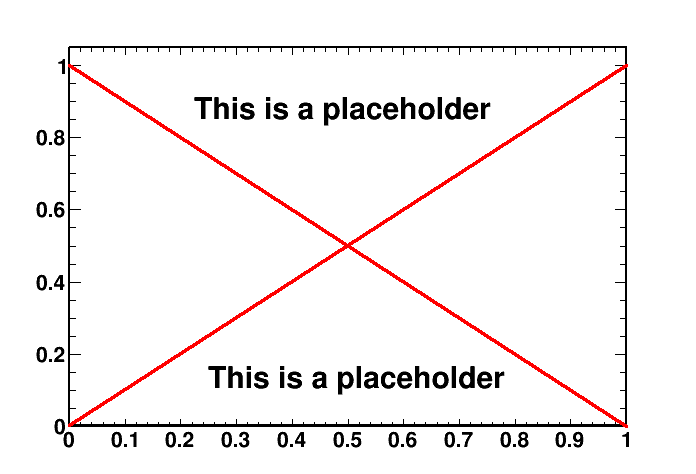
\includegraphics[width=.9\linewidth]{pic/dummy.png}
 \caption{chi2 distribution of first fits (not mines)}
 \label{fig:first_BKGonly_fits}
\end{figure}

Several studies have already tried to see how our predictions of the gamma rays emission and our observations compare. The three main phenomena were modeled as explained to try to recreate the spectrum observed from Earth. The results are clear, there are somethings missing in our interpretation. 
The fit is clearly not working in the galactic plane and the bubbles (as shown on Fig. \ref{fig:first_BKGonly_fits}. The spatial templates used in those fits also show a spherical excess of gamma rays of about 2GeV in the galactic center (GC).

\begin{figure}
 \centering
 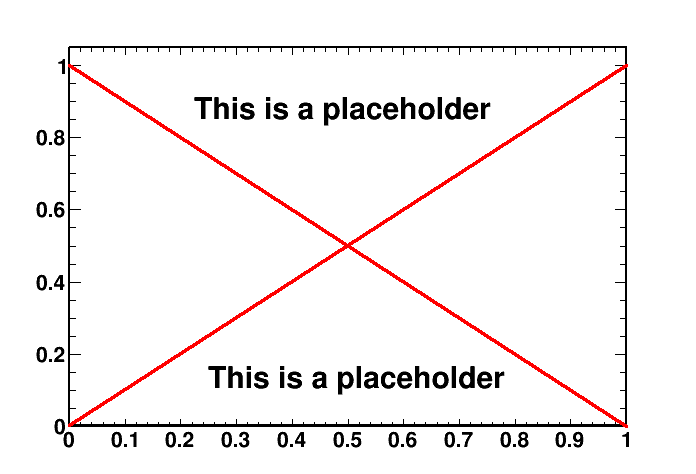
\includegraphics[width=.9\linewidth]{pic/dummy.png}
 \caption{shape of the excess}
 \label{fig:first_BKGonly_fits}
\end{figure}


Two main ideas have emerged to explain this spherical excess.

First is the presence of dark matter in the galaxy in the form of weakly interacting massive particles (WIMP). The spatial distribution of these particles would follow a Navarro-Frrank-White (NFW) profile centered at the GC. They are also expected to produce gamma rays when annihilating with each other via hadrons production. In theory, if the mass of a WIMP particle is around 50GeV, the expected gamma spectrum would peak around 2GeV, where the excess is observed. \todo{cite}
The study of the excess could put strong limits on the mass and annihilation cross section of such WIMP and confirm, or infirm the theory.

The second theory does not involve new physic, but inobserved milli-second pulsars. They would also be spherically distributed around the GC and their gamma spectrum peaks around 2GeV. A few thousands of them would be needed to recreate the intensity of excess. The main default of this explaination resides in the fact that we have observed only a few hundreds? at most. That would requires a very high concentration and a reason why we can not observe them more easely.







































